\documentclass[11pt,a4paper]{article}
\usepackage[margin=2.5cm]{geometry}
\usepackage{amsmath,amssymb}
\usepackage{graphicx}
\usepackage{siunitx}
\usepackage{hyperref}
\usepackage[T1]{fontenc}
\usepackage{lmodern}

\title{02\_Run\_Extraction: Straight-Line Coastdown Interval Detection}
\author{Validation\_Aero\_Test}
\date{\today}

\begin{document}
\maketitle

\section{Overview}
This document describes the straight-line interval detection used to extract
coastdown runs from the cleaned telemetry dataset.  The implementation lives in
\texttt{aero\_validation/segmentation.py} and is invoked via the CLI script
\texttt{Code/02\_Run\_Extraction/export\_drag\_runs.py}.

\paragraph{Pipeline flow}
\begin{center}
\begin{verbatim}
cleaned_10ms.csv  (from 01_Data_Preparation)
    |
    v
export_drag_runs.py    -->  drag_intervals.csv  +  overview plot
    |
    v
generate_run_outputs.py -->  run_XXX.csv  +  per-run QC plots
    |
    v
downstream (drag calculation, 03_Drag_Calculation)
\end{verbatim}
\end{center}

The algorithm:
\begin{itemize}
  \item proposes candidate run starts using speed peak detection,
  \item extends forward until a stopping condition (turning/braking/re-acceleration/stop),
  \item enforces quality gates (straightness, duration),
  \item writes an intervals CSV used by downstream steps.
\end{itemize}

\paragraph{Provenance.}
The example outputs shown in this document are from the Stei\ss{}lingen
aero-validation test day (2025-10-22), comprising 4 stints and 46 extracted
coastdown runs.

\section{Inputs}
From the cleaned dataset CSV produced by the data-preparation pipeline
(see \texttt{01\_Data\_Preparation.pdf}):
\begin{itemize}
  \item \textbf{Time}: \texttt{t\_s} [s]
  \item \textbf{Speed}: \texttt{GPS1\_VEL\_MAG\_ms} [\si{\meter\per\second}]
  \item \textbf{Steering}: \texttt{ICU\_SteeringAngle\_deg} [deg]
  \item \textbf{Optional brakes}: \texttt{ICU\_Brakpresf\_bar}, \texttt{ICU\_Brakpresr\_bar} [bar]
\end{itemize}

\section{Reproducibility}
The following commands reproduce the run extraction from the cleaned dataset
(run from the repository root):

\begin{verbatim}
# Detect coastdown intervals and write the intervals CSV
python Code/02_Run_Extraction/export_drag_runs.py \
    --csv Outputs/01_Data_Preparation/Aero_Validation_Signals_cleaned_10ms.csv \
    --out Outputs/02_Run_Extraction/csv/drag_intervals.csv

# Generate per-run time-series slices and QC plots
python Code/02_Run_Extraction/generate_run_outputs.py \
    --csv Outputs/01_Data_Preparation/Aero_Validation_Signals_cleaned_10ms.csv \
    --intervals Outputs/02_Run_Extraction/csv/drag_intervals.csv \
    --outdir Outputs/02_Run_Extraction/csv
\end{verbatim}

All thresholds can be overridden via CLI flags; see Section~\ref{sec:thresholds}
for the canonical defaults.

\section{Preprocessing}
Let $t$ be the sample times and $v$ the speed signal.
\begin{itemize}
  \item Estimate the median sample period $\Delta t_\mathrm{med}$ from $\Delta t = \mathrm{diff}(t)$.
  \item Convert time windows (seconds) to sample windows by $n \approx \mathrm{round}(\Delta t_\mathrm{window}/\Delta t_\mathrm{med})$.
  \item If smoothing is enabled (default): smooth $v$ with a centered rolling mean using a window derived from \texttt{peak\_window\_s}.
  \item If brake signals exist: combine $b(t)=\max(b_f,b_r)$ and lightly smooth with a centered rolling mean of 5 samples.
\end{itemize}

\section{Candidate peak detection}
Peak detection is implemented in \texttt{detect\_drag\_peaks(t, v, config)}.
It combines two mechanisms and returns sorted unique indices:
\begin{enumerate}
  \item \textbf{Local maxima}: indices where $v_s[i] \ge v_s[i-1]$ and $v_s[i] \ge v_s[i+1]$.
  \item \textbf{Derivative sign change}: indices where the speed derivative changes from clearly positive to non-positive.
\end{enumerate}

\paragraph{Prominence gate}
For each local maximum, compute a prominence proxy using the 60th percentile of
the speed within a local window around the candidate:
\[
  p = v_s[i] - P_{60}(\,v_s\;\text{in a local window around }i\,),
\]
and require $v_s[i] \ge \texttt{min\_peak\_speed}$ and $p \ge \texttt{peak\_prominence}$.

\section{Forward extension and end conditions}
Given a start index $p$ (peak), the algorithm extends forward until the first end condition triggers.
Let $i$ be the current index and $j=i+\texttt{accel\_window\_s}$ (converted to samples).

End conditions (evaluated sequentially):
\begin{itemize}
  \item \textbf{Stop}: $v_s[i] \le \texttt{stop\_speed\_th}$.
  \item \textbf{Turning}: $|\theta[i]| > \texttt{steer\_thresh}$ sustained for \texttt{turn\_window\_s}.
  \item \textbf{Braking}: $b[i] > \texttt{brake\_thresh}$ or an instantaneous brake ``spike'' exceeds \texttt{brake\_spike\_thresh}.
  \item \textbf{Re-acceleration}: if $v_s[j] - v_s[i] > \texttt{reaccel\_eps}$.
\end{itemize}

The returned interval is half-open: $(p,e)$ where $e$ is the first index after the accepted end.

\section{Quality gates}
After computing $(p,e)$:
\begin{itemize}
  \item \textbf{Straightness}: the fraction of samples in $[p,e)$ where $|\theta| \le \texttt{steer\_thresh}$ must be at least \texttt{straight\_ratio}.
  \item \textbf{Duration}: the run duration $t[e-1]-t[p]$ must satisfy \texttt{min\_dur\_s} $\le$ duration $\le$ \texttt{max\_dur\_s}.
  \item \textbf{Non-overlap}: candidate peaks that would overlap a previously accepted interval are skipped.
\end{itemize}

\section{Error handling \& robustness}
\begin{itemize}
  \item \textbf{No peaks found}: if no speed peaks satisfy the prominence and
        minimum-speed gates, an empty intervals CSV is produced (no crash).
  \item \textbf{Missing steering}: if \texttt{ICU\_SteeringAngle\_deg} is absent,
        the straightness gate is skipped and all runs are accepted on duration
        alone.  A warning should be raised in this case.
  \item \textbf{Missing brakes}: if brake pressure channels are absent, the
        braking end-condition is simply not evaluated; runs terminate only on
        stop, turn, or re-acceleration.
  \item \textbf{Short dataset}: if fewer than 3 samples exist, segmentation
        returns an empty list immediately.
\end{itemize}

\section{CLI usage and outputs}
\subsection*{Export intervals}
\texttt{Code/02\_Run\_Extraction/export\_drag\_runs.py} loads the cleaned
dataset, runs segmentation, writes an intervals CSV, and generates an overview
plot.

Default output paths:
\begin{itemize}
  \item Intervals CSV: \texttt{Outputs/02\_Run\_Extraction/csv/drag\_intervals.csv}
  \item Overview plot: \texttt{Outputs/02\_Run\_Extraction/plots/velocity\_overview\_with\_runs.png}
\end{itemize}

\begin{figure}[ht]
  \centering
  \includegraphics[width=\linewidth]{../../Outputs/02_Run_Extraction/plots/velocity_overview_with_runs.png}
  \caption{Overview of detected coastdown intervals overlaid on the speed trace (generated by \texttt{export\_drag\_runs.py}).}
\end{figure}

Intervals CSV schema (key fields):
\begin{itemize}
  \item \texttt{run\_id}: 1..N
  \item \texttt{start\_idx}, \texttt{end\_idx}: index range into the input dataset (end exclusive)
  \item \texttt{t0\_s}, \texttt{t1\_s}, \texttt{duration\_s}
  \item \texttt{v\_start\_ms}, \texttt{v\_end\_ms}
  \item \texttt{source\_basename}, \texttt{row\_count}: metadata for mismatch detection
\end{itemize}

\subsection*{Optional debug log}
If \texttt{--debug-out} is provided, \texttt{segment\_drag\_runs\_with\_debug}
writes a per-peak decision log with the following columns:
\begin{center}
\begin{tabular}{ll}
\texttt{peak\_idx}     & Index of the candidate peak \\
\texttt{t\_peak}       & Time at the peak [s] \\
\texttt{accepted}      & Boolean: did this peak yield a valid run? \\
\texttt{reason}        & Rejection reason if not accepted
                         (\texttt{overlap}, \texttt{duration}, \texttt{straight}) \\
\texttt{start\_idx}    & Start index of the accepted interval \\
\texttt{end\_idx}      & End index (exclusive) \\
\texttt{t0}, \texttt{t1} & Start and end times [s] \\
\texttt{duration}      & Run duration [s] \\
\texttt{steer\_ratio}  & Fraction of samples within steering threshold \\
\texttt{end\_reason}   & What ended the run
                         (\texttt{stop}, \texttt{turn}, \texttt{brake},
                          \texttt{brake\_spike}, \texttt{reaccel}) \\
\end{tabular}
\end{center}

\section{Default thresholds}
\label{sec:thresholds}
The canonical defaults are defined in the \texttt{DragRunConfig} dataclass
(\texttt{aero\_validation/segmentation.py}) and can be overridden individually
via CLI flags or programmatically by passing a custom instance.

The defaults exposed by \texttt{export\_drag\_runs.py} are:
\begin{center}
\begin{tabular}{ll}
\texttt{steer\_thresh} & 10 deg \\
\texttt{straight\_ratio} & 0.75 \\
\texttt{min\_peak\_speed} & 15.0 m/s \\
\texttt{peak\_window\_s} & 0.5 s \\
\texttt{peak\_prominence} & 0.05 m/s \\
\texttt{reaccel\_eps} & 0.2 m/s \\
\texttt{accel\_window\_s} & 0.5 s \\
\texttt{brake\_thresh} & 0.05 bar \\
\texttt{brake\_spike\_thresh} & 0.1 bar/s \\
\texttt{turn\_window\_s} & 0.3 s \\
\texttt{min\_dur\_s} & 1.5 s \\
\texttt{max\_dur\_s} & 20.0 s \\
\texttt{stop\_speed\_th} & 0.2 m/s \\
\end{tabular}
\end{center}

\section{Per-run outputs}
The script \texttt{Code/02\_Run\_Extraction/generate\_run\_outputs.py} consumes
\texttt{drag\_intervals.csv} and writes:
\begin{itemize}
  \item \texttt{Outputs/02\_Run\_Extraction/csv/run\_\{XXX\}.csv}: sliced time series per interval
  \item \texttt{Outputs/02\_Run\_Extraction/plots/run\_\{XXX\}\_velocity\_steering\_brake.png}: QC plots per run
\end{itemize}

\begin{figure}[ht]
  \centering
  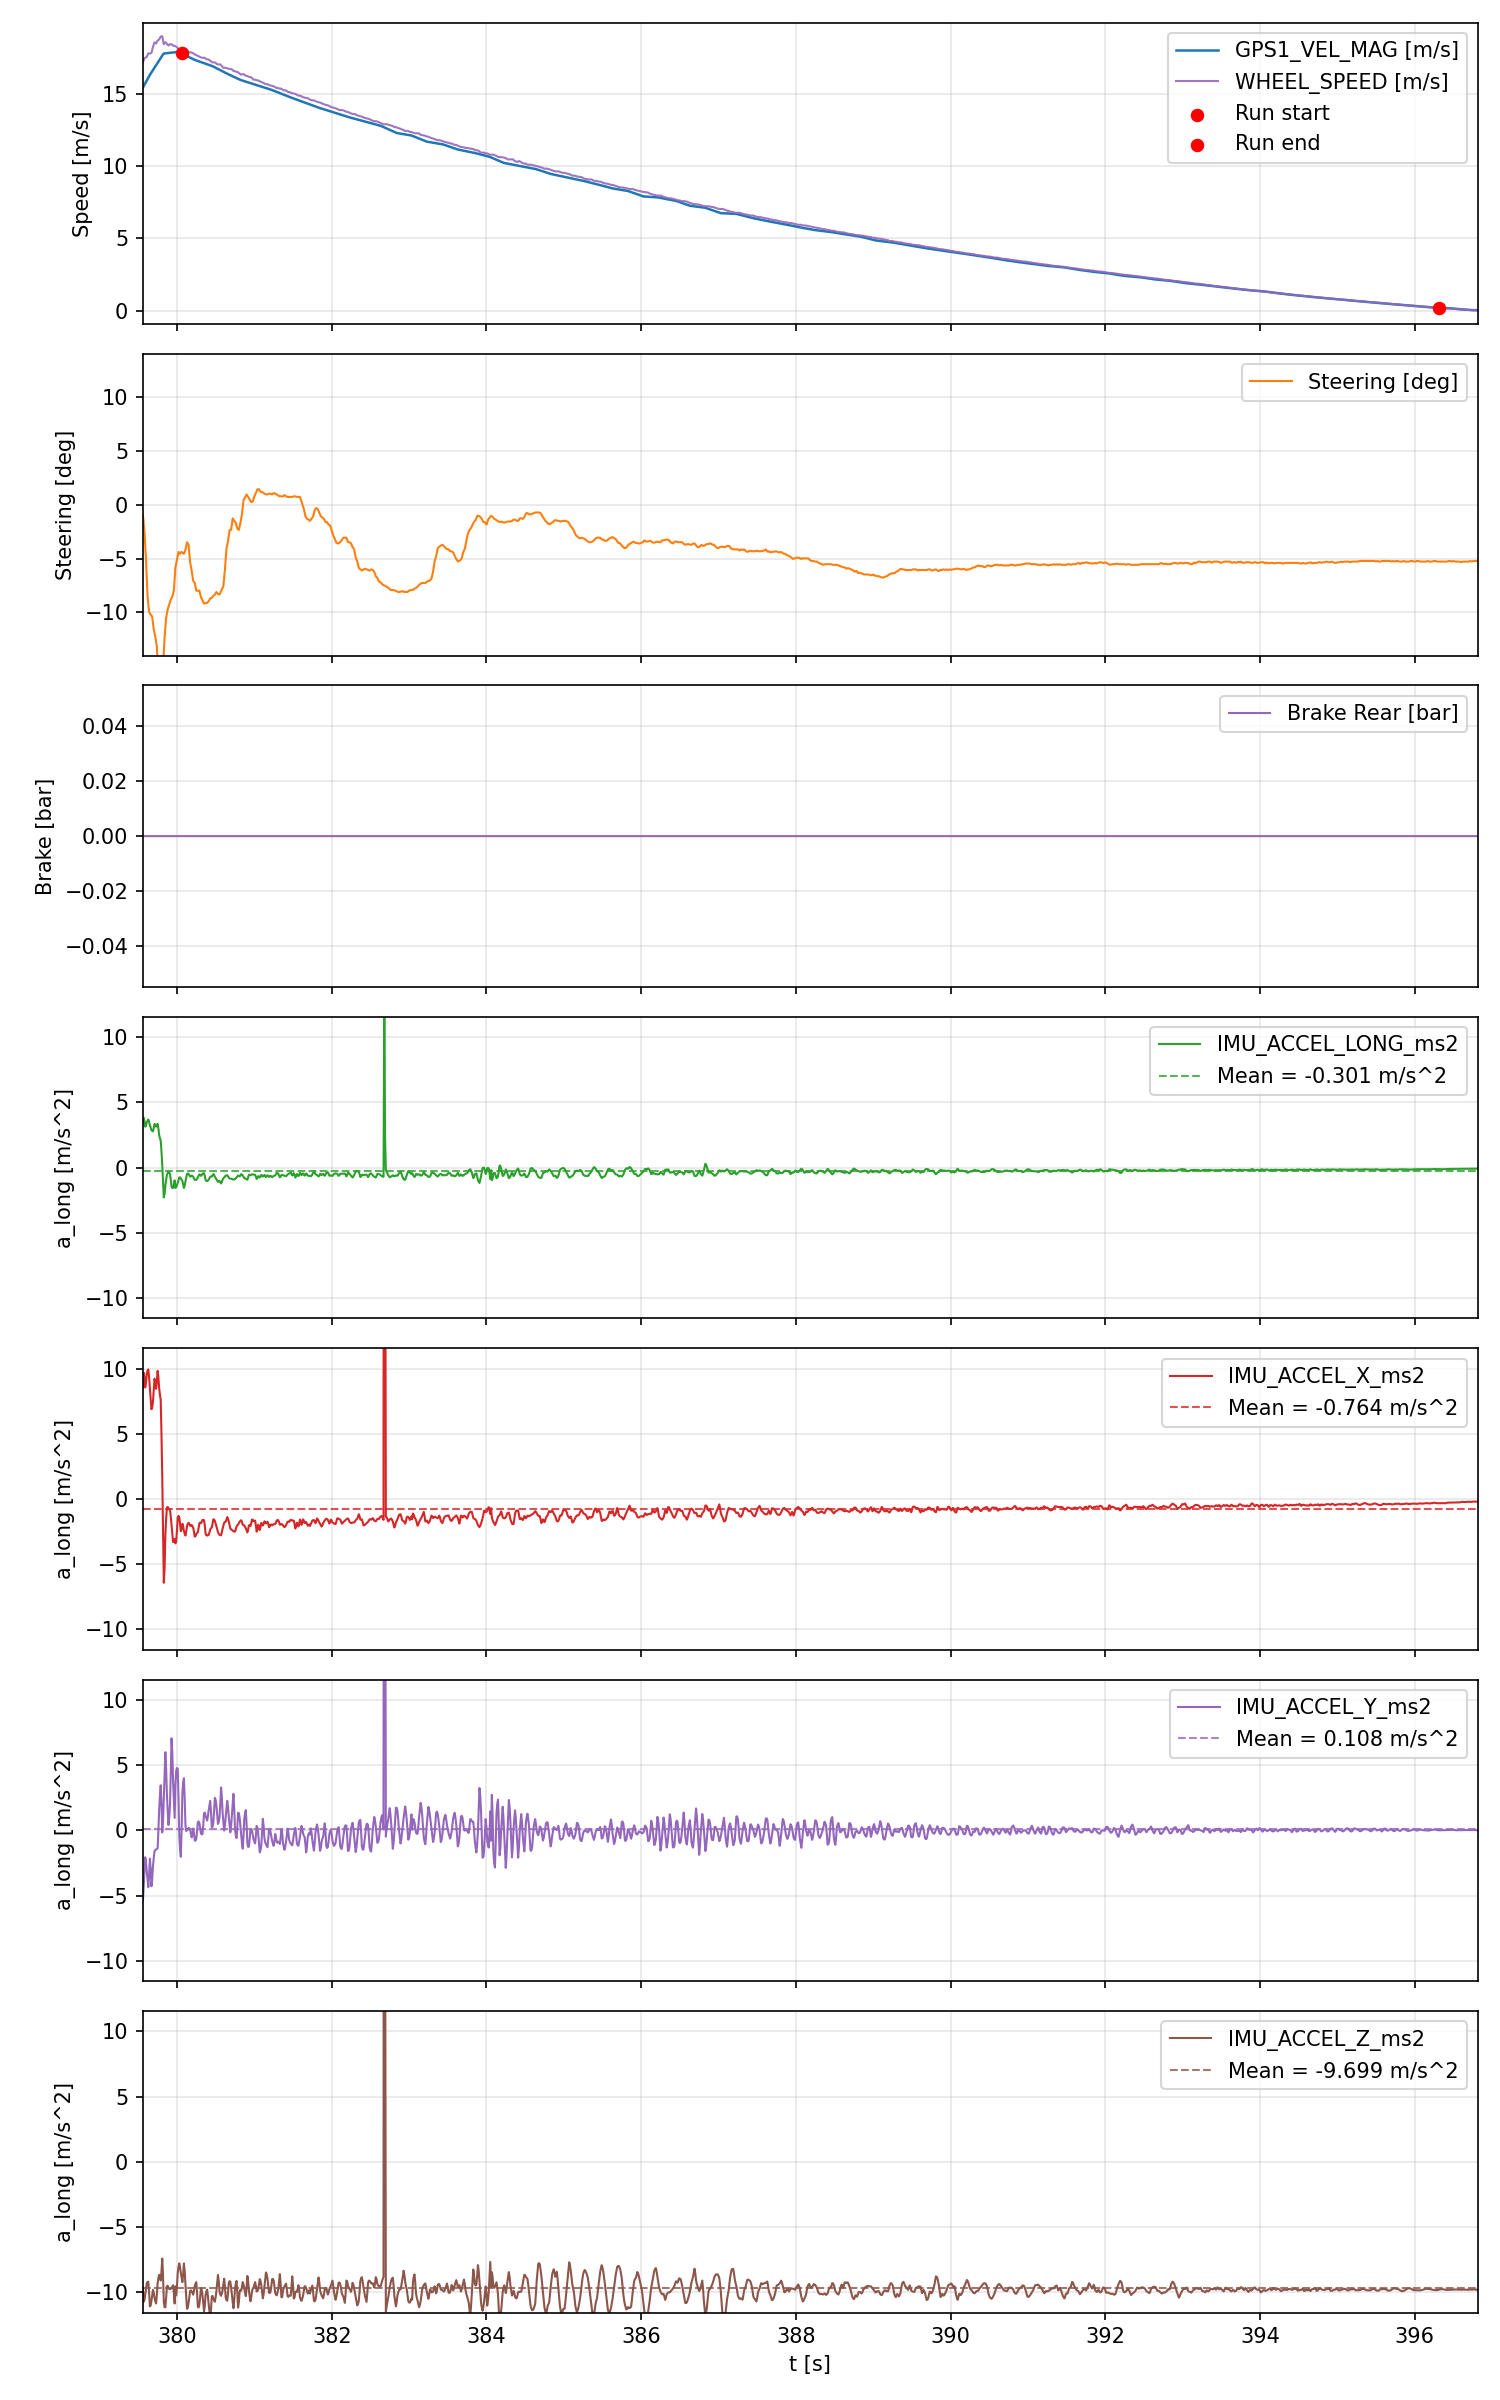
\includegraphics[width=\linewidth]{../../Outputs/02_Run_Extraction/plots/run_001_velocity_steering_brake.png}
  \caption{Example per-run QC plot (speed, steering, and brake traces) for Run~001.}
\end{figure}

The intervals CSV produced here is the input for the drag coefficient
estimation step (see \texttt{03\_Drag\_Calculation.pdf}).

\end{document}
